\documentclass[a4paper,10pt]{article}
\usepackage[margin=2.5cm]{geometry}
\usepackage[utf8]{inputenc}
\usepackage[colorlinks=true,urlcolor=blue]{hyperref}
\usepackage{amsmath}
\usepackage{graphicx}
\usepackage{float}
\usepackage{caption}

\usepackage{listings} %Alternative to minted



\setlength{\parindent}{0em}
\setlength{\parskip}{1em}

\title{\textbf{Deep Learning for Image Analysis} 
\\ DL4IA -- Report for Assignment 1}
\author{Student Linus Falk}
\date{\today}

\begin{document}

\maketitle

\section{Introduction}
First assignment in the course Deep learning for image analysis

\section{Mathematical exercises}

Given the linear regression model:
\begin{equation}
    z_i = \sum_{j=1}^p w_jx_{ij} + b 
\end{equation}

with the cost function 
\begin{equation}
\label{eq:cost}
\begin{split}
    J = \frac{1}{n}\sum_{i=1}^nL_i \\
    \text{where } L_i = (y_i-z_i)^2    
\end{split}
\end{equation}






\textit{\textbf{Exercise 1.}}
\begin{equation*}
    \frac{\partial J} {\partial w_j} = \frac{1} {n} \sum_{i=1}^{n} \frac{\partial J} {\partial z_i}  \frac{\partial z_i} {\partial w_j} 
\end{equation*}

\begin{equation*}
   \frac{\partial J} {\partial b}  = \frac{1} {n} \sum_{i=1}^{n} \frac{\partial J} {\partial z_i}  \frac{\partial z_i} {\partial b} 
\end{equation*}


\textit{\textbf{Exercise 2.}}

\begin{equation*}
\begin{split}
    \frac{\partial J}{\partial z_i} = \frac{1} {n} \sum_{i=1}^{n}  2(L_i) \\
    \frac{\partial z_i} {\partial b} = \frac{\partial} {\partial b}  \sum_{j=1}^p (w_jx_{ij}+b) = 1 \\
    \frac{\partial z_i} {\partial w_j} = \frac{\partial} {\partial w_j} \sum_{j=1}^p (w_jx_{ij}+b) = \sum_{j=1}^p x_{ij}
\end{split}
\end{equation*}


\section{Code exercises}

For exercises where you are asked to write code, include the important functions and steps that you have implemented. For functions it is good practise to always have a small description in the beginning of the function, explaining what the function does, what the arguments are and what is returned. In \LaTeX\ you can for instance use the \emph{minted} package to include code 
%(read more about listings \href{https://www.overleaf.com/learn/latex/code_listing}{here}).
(read more about minted \href{https://www.overleaf.com/learn/latex/Code_Highlighting_with_minted}{here}).


\hfill \break
\textit{\textbf{Exercise 3.} Implement a gradient descent algorithm ...}

Based on the derivations given in exercise 1 and 2, the following functions are implemented to perform gradient descent for linear regression. 

\begin{itemize}
\item
The \emph{initialize} function is used to initialize the weights and offsets by method X.
\item
The \emph{cost} function takes \ldots and \ldots as input and calculates the cost according to eq. \eqref{eq:cost}.
\end{itemize}

\begin{lstlisting}[frame=lines,framesep=2mm]{language=python}

def initialize(arg1, arg2, ...):
    """ param arg1: description of argument 1
        param arg2: description of argument 2
        ...s
        
        return: description of what the function returns
    """
    
    w = ...
    b = ...
    
    
    return w, b

def cost(arg1, arg2, ...):
    """ param arg1: description of argument 1
        param arg2: description of argument 2
        ...
        
        return: description of what the function returns
    """
    
    J = 
    
    return J

\end{lstlisting}

\newpage
\hfill \break
The weights and offsets are optimized to minimize the cost as follows:

\begin{lstlisting}[frame=lines,framesep=2mm]{language=python}

w,b = initialize(*args) #Initialize weights and offsets
n_iterations = 1000 #Number of gradient descent iterations

for it in range(n_iterations):
    
    ...
    
    J = cost(*args)
\end{lstlisting}


\section{Results}
When presenting results, include plots of the optimization process, quantitative scores for your models and other relevant stuff to show the performance of your models. An easy to use and well documented library in python is \emph{Matplotlib} (\href{https://matplotlib.org/}{link}). 
For plots, \textbf{always} write a caption explaining what is shown in the plot, and also what can be observed/concluded from the plot. Remember to always have labels on the axes, and when suitable a legend (if multiple plots in same figure). Make the plots of a suitable size to be visible (if printed). See Figure \ref{fig:cost_per_iteration} for an example.


\begin{figure}[H]
 \centering
    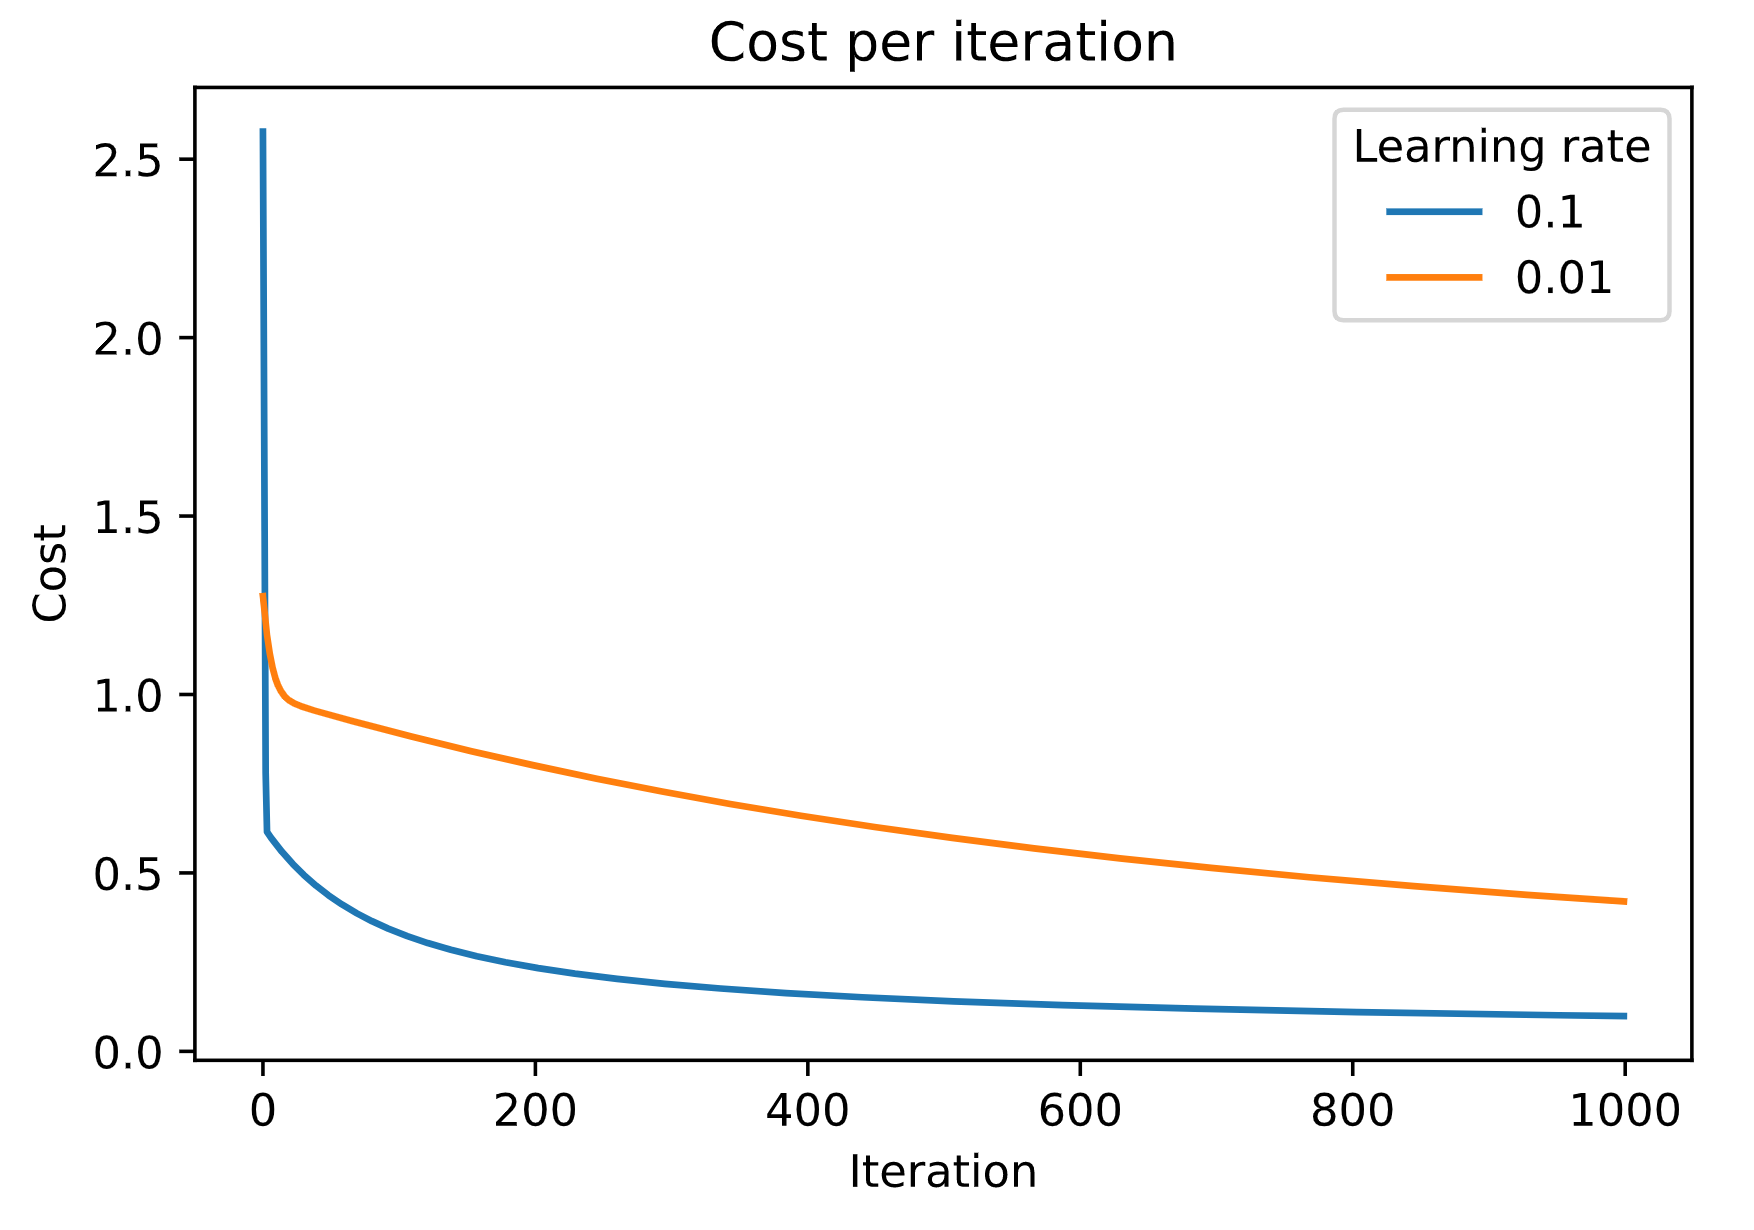
\includegraphics[width=0.6\textwidth]{figures/cost_per_iteration_lr.png}
    \caption{Plot showing how the cost \eqref{eq:cost}, evaluated on the training sets, is changing with with number of iterations. It can be seen that\ldots}
    \label{fig:cost_per_iteration}
\end{figure}



\begin{thebibliography}{1}

\bibitem{Adams} Adams, Douglas (1979). The Hitchhiker's Guide to the Galaxy. Pocket Books. p. 3.

\end{thebibliography}

\end{document}
